\documentclass[11pt]{article}
\usepackage[a4paper,margin=1.8cm]{geometry}
\usepackage{graphicx,amsmath,microtype}
\usepackage[colorlinks=true,linkcolor=blue]{hyperref}
\usepackage{fancyhdr}
\pagestyle{fancy}\fancyhf{}
\fancyhead[L]{\small graphMoDE: completed spiral-panel comparison}
\fancyhead[R]{\small 17 September 2026}
\fancyfoot[L]{\small Single development panel; saved c5 draws}
\fancyfoot[R]{\small\thepage}
\setlength{\headheight}{15pt}
\setcounter{figure}{3}
\begin{document}
\begin{figure}[!ht]
\centering
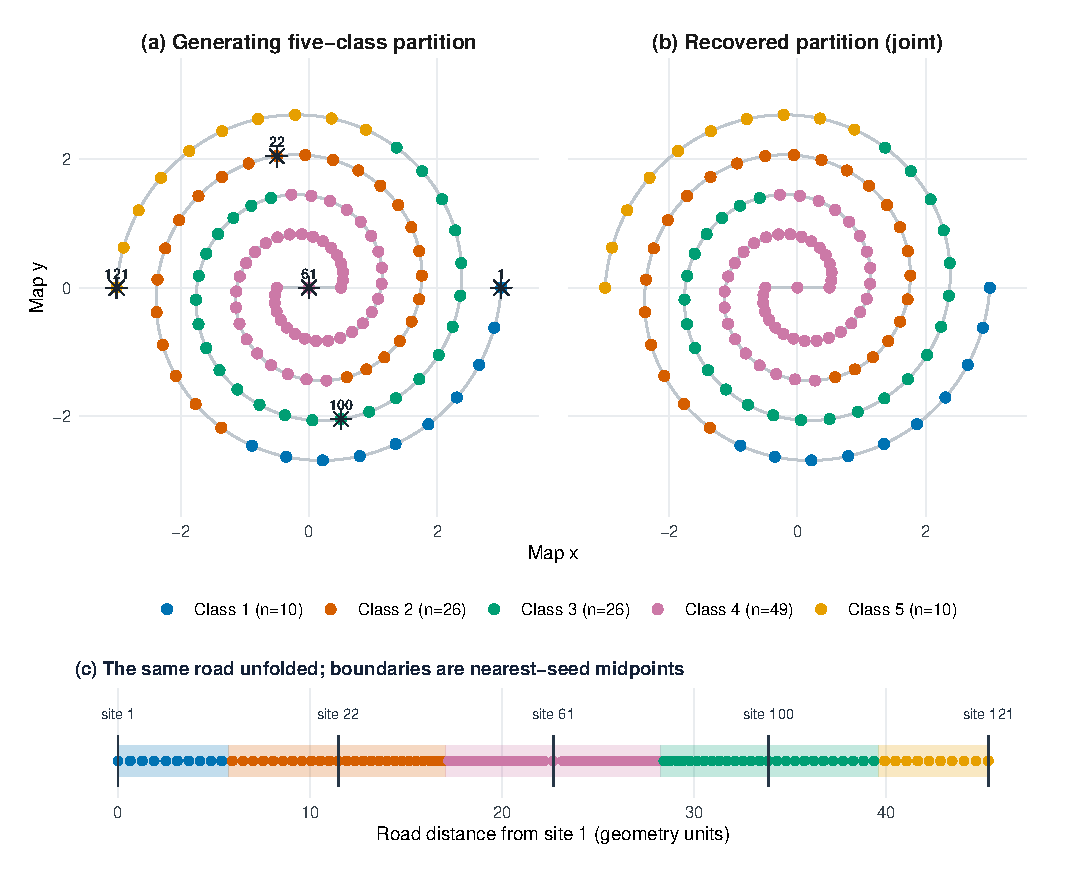
\includegraphics[width=1.0\textwidth]{figures/graphMoDE-c5-classification.pdf}
\caption{Five-class generation and recovery on the intertwined-spiral road.
(a) Colors denote the five generating profiles; stars mark the five
road-distance Voronoi seeds, annotated by geometric site ID. Gray curves
are the physical roads, including the central connector.
(b) The first retained partition of joint chain 1 (sweep 301), with labels
aligned to the generating colors only for display. This draw was not
selected by its recovery score: all 1,200 retained joint partitions give
the same grouping, recovering all 121 sites with fitted capacity ten.
(c) The connected road unfolded by distance from site 1; colored intervals
show the nearest-seed cells. Class sizes are 10, 26, 26, 49 and 10 in
profile-label order. Distance and map coordinates use geometry units.}
\label{fig:c5-partition}
\end{figure}

\clearpage
\begin{figure}[!ht]
\centering
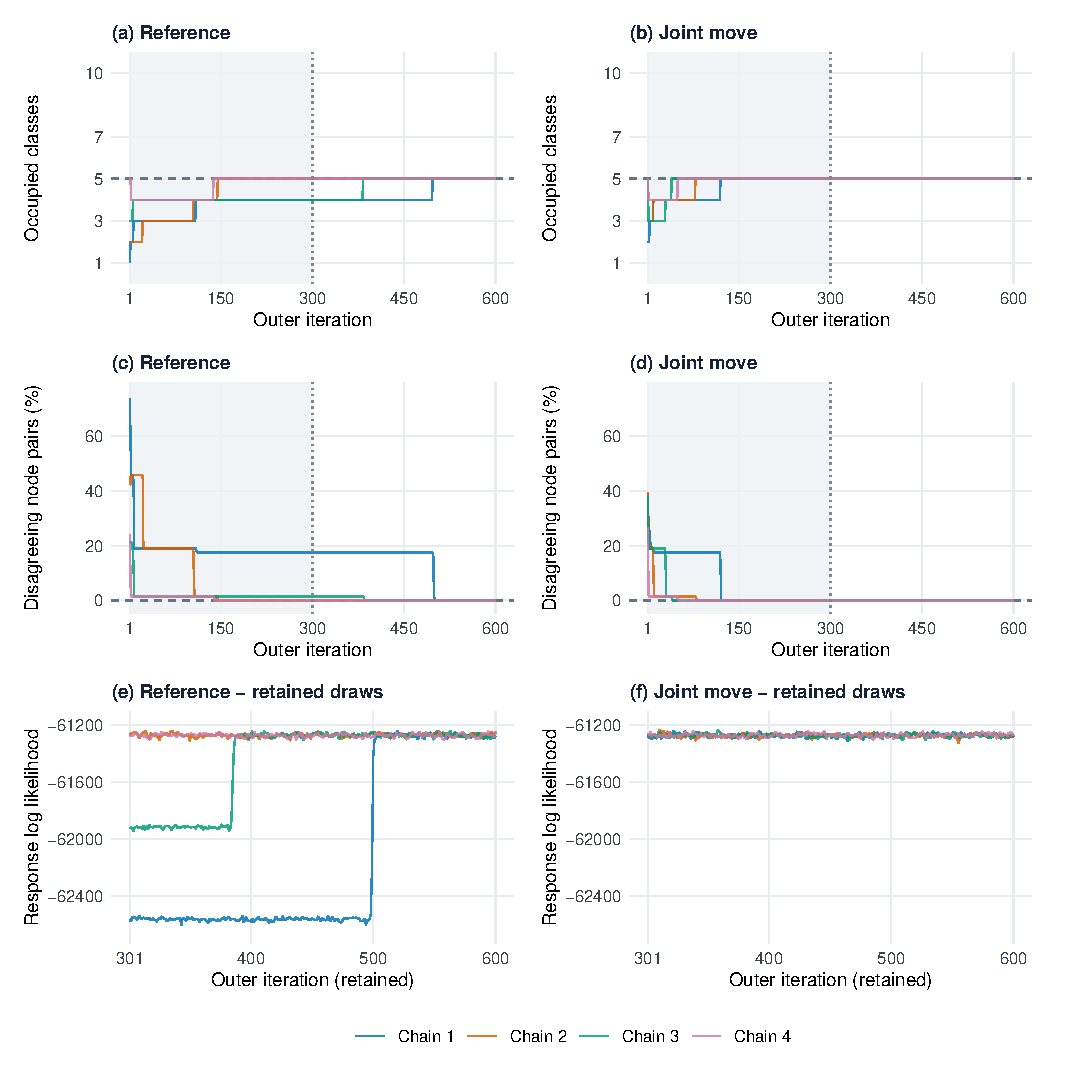
\includegraphics[width=1.0\textwidth]{figures/graphMoDE-c5-traces.pdf}
\caption{Saved traces for the reference and joint-move arms on the same
development panel. Colors identify four chains within each arm.
The upper rows show occupied classes and the percentage of unordered
site pairs whose co-membership differs from truth, for sweeps 1--600;
gray shading marks the first 300 sweeps discarded as warm-up. Dashed
horizontal lines mark five classes and zero pair disagreement. Traces
begin after the first sweep, following the registered 1-, 3-, 7- and
10-class starts. The bottom row shows total response log likelihood for
retained sweeps 301--600 only. Each row uses the same vertical scale
across arms. The joint chains reach the correct partition before warm-up
ends; two reference chains reach it during retention. Stable classification
does not imply that every continuous-parameter check passes.}
\label{fig:c5-traces}
\end{figure}

\clearpage
\begin{figure}[!ht]
\centering
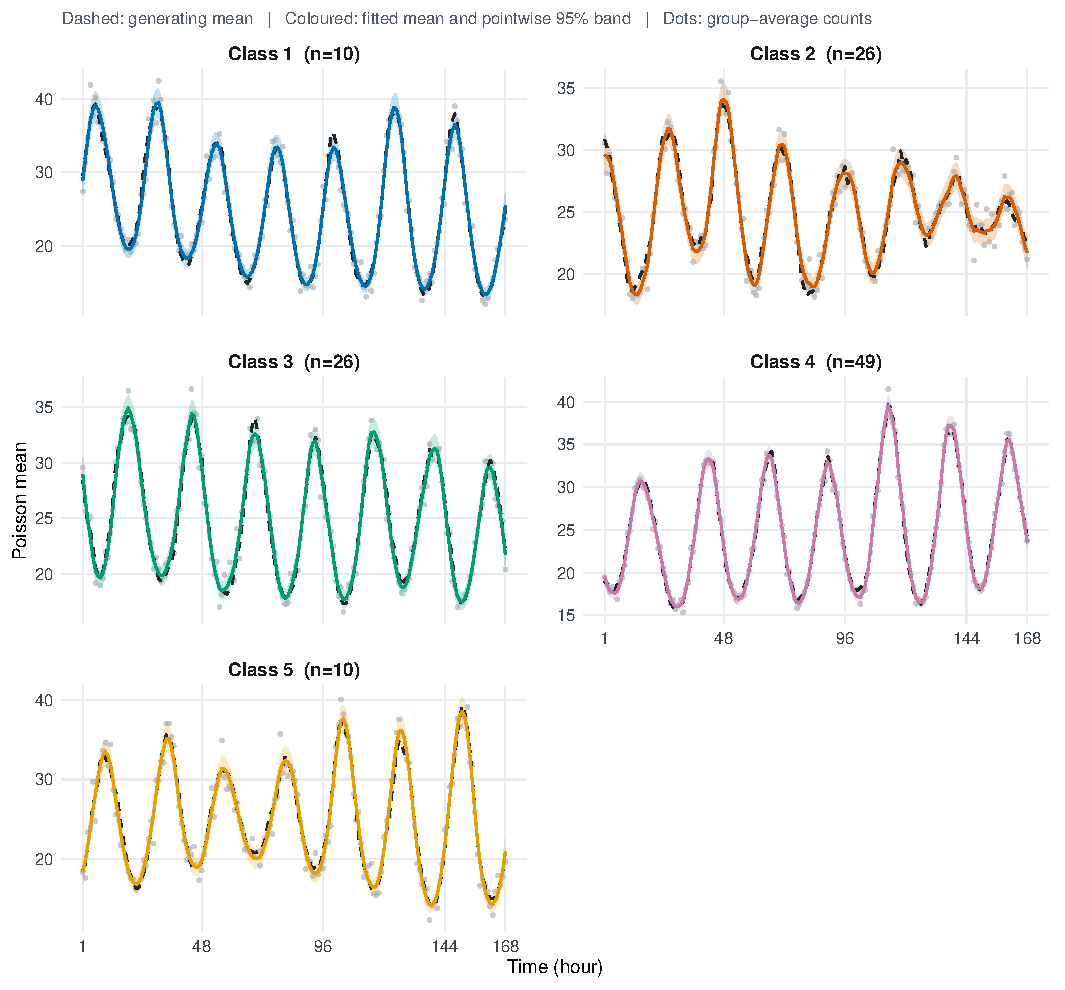
\includegraphics[width=1.0\textwidth]{figures/graphMoDE-c5-profiles.pdf}
\caption{Generating and fitted temporal profiles for the five recovered
classes in the joint arm. Dashed black curves are the generating Poisson
means; colored curves are means of the saved latent-mean draws. Shading
gives pointwise 2.5th--97.5th percentiles pooled over four chains with
300 retained draws each. Gray dots are observed counts averaged over
sites in each generating class. Class colors match the partition map,
and vertical scales vary by class. These are empirical summaries of
latent means from the development run, not prediction intervals for
future counts or evidence of calibrated interval coverage. The retained
draws are correlated and the full convergence rule remains unmet.}
\label{fig:c5-profiles}
\end{figure}

\clearpage
\begin{figure}[!ht]
\centering
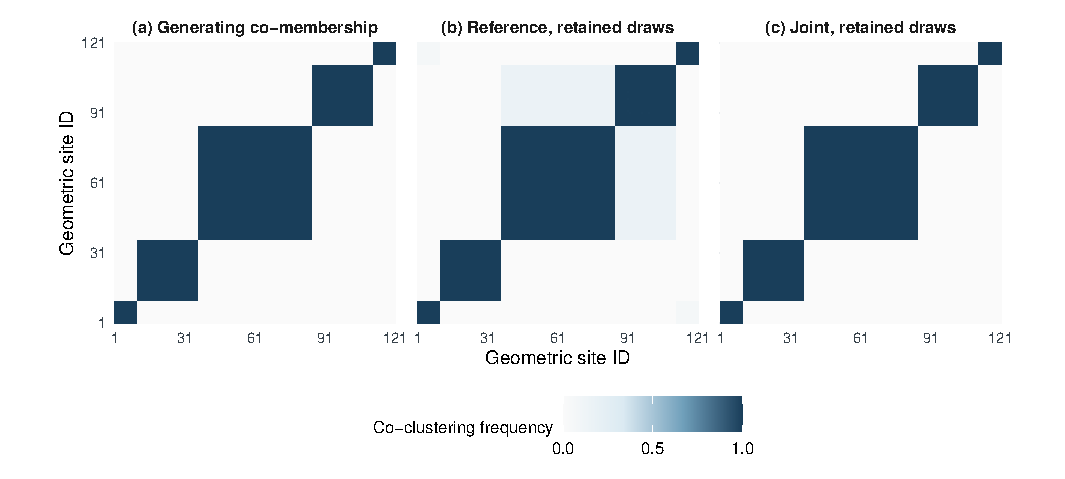
\includegraphics[width=1.0\textwidth]{figures/graphMoDE-c5-psm.pdf}
\caption{Co-clustering summaries for the single development panel.
(a) The generating co-membership matrix; (b,c) empirical posterior
similarity matrices for the reference and joint arms, averaging the
same-class indicators over all four chains and all 300 retained draws
per chain. Both axes follow geometric site IDs 1--121, in the same order
for all panels. The joint matrix equals the generating matrix exactly;
the reference matrix retains the effect of delayed partition recovery
in two chains. Empirical frequencies zero or one describe these saved
draws and do not demonstrate that all competing partitions were explored.}
\label{fig:c5-psm}
\end{figure}

\clearpage
\begin{figure}[!ht]
\centering
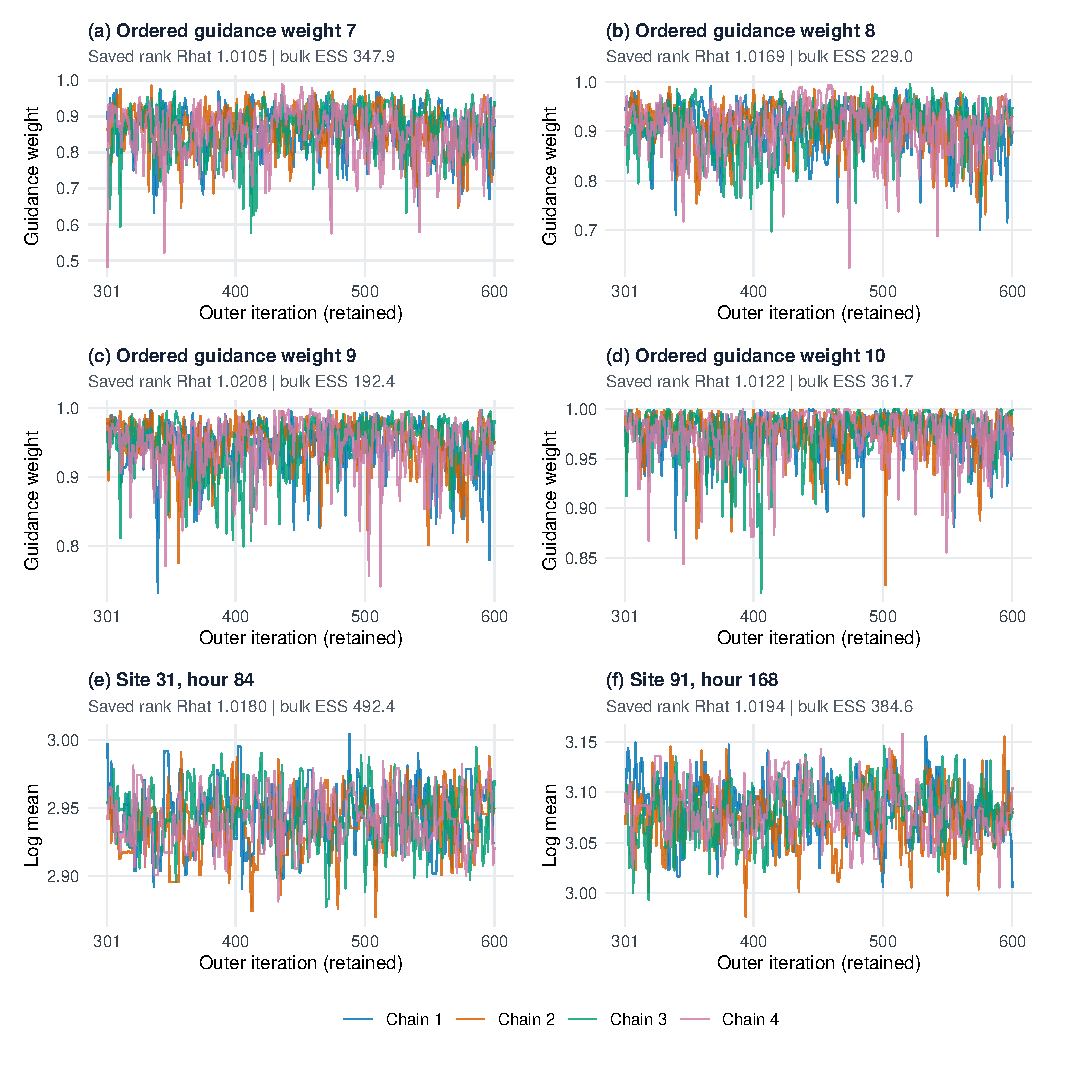
\includegraphics[width=0.98\textwidth]{figures/graphMoDE-c5-residual-traces.pdf}
\caption{Retained traces of all six nonconstant scalar summaries that
failed the joint arm's original diagnostic rule. The upper four panels
show the seventh through tenth order statistics of the ten guidance
weights, not fixed expert labels; the lower two show unit log means at
the stated geometric site IDs and hours. Four chain colors are used
throughout. Rank-normalized split $\widehat R$ and bulk effective sample
sizes in the panel headings are copied from the completed run's saved
diagnostics, not recomputed for this figure. The unchanged rule requires
both rank and folded $\widehat R\leq1.01$ and bulk/tail effective sample
sizes of at least 400. All retained sweeps 301--600 are shown.}
\label{fig:c5-residual-traces}
\end{figure}

\clearpage
\end{document}
